\documentclass{article}

\usepackage{amsmath}
\usepackage{fancyhdr}
\usepackage{graphicx}
\graphicspath{{}}

%% some colours
\usepackage{color}
\definecolor{deepblue}{rgb}{0,0,0.5}
\definecolor{deepred}{rgb}{0.6,0,0}
\definecolor{deepgreen}{rgb}{0,0.5,0}
\definecolor{backcolour}{rgb}{0.95,0.96,0.93}

%%%%%%%%%%%%%% CODE STUFF %%%%%%%%%%%%%%
%%%%%%%%%%%%%%%%%%%%%%%%%%%%%%%%%%%%%%%%
\usepackage{cprotect} % to be used in sol
\usepackage{listings} % for code display
% setting code style
\newcommand\pythonstyle{\lstset{
        language=Python,
        backgroundcolor=\color{backcolour},
		basicstyle=\footnotesize,
		otherkeywords={self},
		keywordstyle=\footnotesize\color{deepblue},
		emph={__init__},
		emphstyle=\footnotesize\color{deepred},
		stringstyle=\color{deepgreen},
		frame=single,
		showstringspaces=false  ,
		breaklines=true,
		numbers=left,
		numberstyle=\footnotesize,
		tabsize=4,
		breakatwhitespace=false
	}}

% Python environment
\lstnewenvironment{python}[1][]{
    \pythonstyle
    \lstset{#1}
}{}

% Python for external files
\newcommand\pythonexternal[2][]{{
    \pythonstyle
    \lstinputlisting[#1]{#2}
}}

% Python for inline
\newcommand\pythoninline[1]{{\pythonstyle\lstinline!#1!}}

%%%%%%%%%%%%%%%%%%%%%%%%%%%%%%%%%%%%%%%%
% setting the style for ex documents
\pagestyle{fancy}
\fancyhf{}
\fancyhead[L]{\thetitle}
\fancyhead[C]{}
\fancyhead[R]{\theauthor}
\renewcommand{\headrulewidth}{0.4pt} %obere Trennlinie
\fancyfoot[L]{Due: \thedate}
\fancyfoot[R]{\thepage} %Seitennummer
\renewcommand{\footrulewidth}{0.4pt}

% include solutions
\newcommand\sol[1]{{\large\textbf{\\Solution:}}#1}
\usepackage{setspace}

\title{BPP Exercise 8 - OOP}
\author{A. Hain, M. Nipshagen}
\date{04.06.2018, 12:00}

\makeatletter
\let\thetitle\@title
\let\theauthor\@author
\let\thedate\@date
\makeatother


\newcommand\itemsub[1]{
	\begin{itemize}
		\item #1
	\end{itemize}
}

% do not include solutions
% \renewcommand\sol[1]{}


\begin{document}

The deadline for this exercise sheet is \textbf{Monday, \thedate.}

\section*{Introductory Words}
Remember that from this homework onwards, you need proper documentation to pass
the homework. The documentation doesn't need to be \textit{perfect}, but
everything that needs a docstring, should have a docstring.


\section{Warm-Up: The Land Before Time}
Many many years ago, our planet was the habitat of many different types of dinosaurs.\\
We modeled several kinds of them and their behavior (in a manner that may or may
not be a little simplified) in a file named \texttt{dinos.py}.\\
Look at the dino classes given in the file. State for each class the following:
\begin{itemize}
	\item{All superclasses}
	\item{All subclasses}
	\item{All classes it extends}
	\item{All functions it can use}
	\item{All functions it overrides}
\end{itemize}

\FloatBarrier
\begin{figure}[ht!]
	\centering
	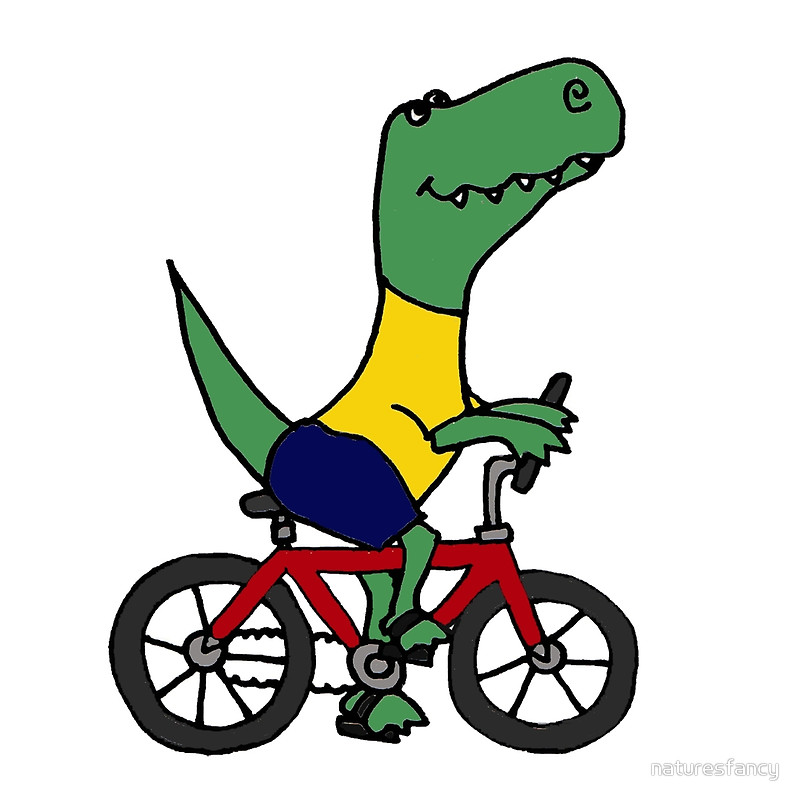
\includegraphics[width=.8\textwidth]{dino_bike}
	\caption{Somewhat related to the task at hand.}
	Taken from naturesfancy at redbubble
	\url{https://www.redbubble.com/de/people/naturesfancy/works/16720425-cute-t-rex-dinosaur-riding-red-bicycle}
\end{figure}
\FloatBarrier

\section{I want to ride my bicycle, I want to ride my bike}
Implement three classes: \textit{Bike}, \textit{Bicycle} and \textit{Motorbike}.\\
\textit{Bike} is the superclass of both \textit{Bicycle} and \textit{Motorbike}.\\
A \textit{Bike} has a number of seats and a number of gears. It can start being ridden and
end being ridden. Also, one is able to change the gears (to a gear number that
actually exists.)\\
Additionally to the \textit{Bike} functions, a bell on the \textit{Bicycle} can be rung.\\
A \textit{Motorbike}, additionally to the \textit{Bike}, has a tank that can be
either full or empty. When you ride the \textit{Motorbike}, the tank is empty afterwards.\\
Write a module of the classes according to the description and add another module
that tests them with some values.\\
Think about which of your attributes need to be public and which should be set private.\\
Don't forget to include proper documentation!

\noindent\textit{Note:} There is not only one solution. Your solution (e.g. the bell) can
be more or less complex depending on how complex you want it to be.

\section{To Battle}
Let's play a game! In the .zip archive you will find the file \texttt{battle.py}.
In this file, we implemented a game loop that has two knights battle. But there
is no knight template yet, and this is where you come in!\\
The basic concept of battle is as follows: Each player is asked to create a knight,
which consists of a name and attribute points (more on that below). Then one player
is chosen at random to have the first turn. Each turn the remaining health of the
players is displayed. The active player can choose an action (an attack)
to perform, and the other player will take damage accordingly. This loop repeats
for as long as both players are alive. After that the winning player is displayed,
and you can choose to play another round.

\noindent Familiarise yourself with the code in \texttt{battle.py} to some extent. We tried to 
document it thoroughly, so the code is (hopefully) well understandable, but if you
struggle with understanding the code just send us a message, and also you
\textit{do not} have to understand the code in full extent to do this homework. So do not
worry if you cannot follow the code line by line.\\
You will also find the module \texttt{util} in the .zip. Make sure that it is in the same folder
as the battle module, when running it. It contains two utility functions that unnecessarily
bloated the battle code.\\

\noindent Every knight has the attributes \textit{vitality, strength and luck} and a 
fixed amount of attribute points, that they can spend on their attributes.
They always have to use all of their attribute points. You can freely
choose how many attribute points your knights have (but all knights have the same).\\
The detailed outline of the class is below.\\

\noindent Your task is to write a module named \texttt{knights}. This module shall fullfill
the following requirements:
\begin{itemize}
	\item \texttt{MAX\_ATTRIBUTE\_POINTS}: a constant integer that holds how many
		attribute points a knight has
	\item \texttt{ATTRIBUTES}: a constant list that holds all attribute names
		as strings, in the same order they appear in the constructor
	\item \texttt{KnightError}: A special exception that is thrown when there is
		an error knighting a new knight. All custom errors extend the 
		\texttt{Exception} class. This custom error needs no properties, nor
		methods (not even \texttt{\_\_init\_\_}). It is enough to extend \texttt{Exception}.
	\item \texttt{Knight}: The very important class. This is the template for all our
		knights that we are going to send into battle.
\end{itemize}
Now, onto the important part: The \textbf{Knight class}. A knight instance is initialised with
a \textbf{name}, the \textbf{vitality} attribute points, the \textbf{strength} points, and the
\textbf{luck} points. The class needs to implement:
\begin{itemize}
	\item \textbf{properties}: \texttt{name, health, strength, luck, crit\_modifier, available\_actions}
		\begin{itemize}
			\item \texttt{name}: the name of the knight
			\item \texttt{health}: this should be a property of the knight, which is read-only.
				The only way this is altered is through the \texttt{take\_damage}
				function. It should be initialised to the \textit{floored integer} value of
				$vitality * 1.5$, where \texttt{vitality} is the passed parameter on initialisation.
			\item \texttt{strength}: the points this knight has in strength
			\item \texttt{luck}: the points this knight has in luck, multiplied by 2.
				This is the critical hit chance in percent.
			\item \texttt{crit\_modifier}: The amount the attacks are multiplied with when they
				critically strike. We chose 3 for this.
			\item \texttt{available\_actions}: A list of all available actions this knight can take.
				Note that this should be a list of \textit{functions} and not of strings, or other
				types.
		\end{itemize}
	\item \texttt{\_\_init\_\_()}: this one should be mostly clear. It also should
		throw a \texttt{KnightError} if the sum of all attribute arguments are
		unequal to the set \texttt{MAX\_ATTRIBUTE\_POINTS} -- so either if it is
		below or above.
	\item \texttt{alive()}: a function that returns whether the knight is 
		still alive. The knight dies when their health is or falls below 0.
	\item \texttt{light\_attack()}: A lighter attack with smaller damage and a higher
		critical strike chance. The damage is calculated by taking the \textit{floored integer}
		value of the formula: $1 + 0.15 * strength$. If the hit was a critical hit, the 
		damage is multiplied by the \texttt{crit\_modifier} before flooring it. The critical
		chance is doubled for the light attack.\\
		The function returns a tuple consisting of the damage and a boolean whether the attack
		was critical, in this order.
	\item \texttt{heavy\_hit()}: A heavier attack with higher damage, but lower critical chance.
		The damage is calculated by taking the \textit{floored integer} value of the formula
		$3 + 0.4 * strength$.If the hit was a critical hit, the damage is multiplied by
		the \texttt{crit\_modifier} before flooring it.\\
		The function returns a tuple consisting of the damage and a boolean whether the attack
		was critical, in this order.
	\item \texttt{all\_actions()}: This function should return the list of all actions this knight
		can take.
	\item The string method should return only the name of the knight.
\end{itemize}

\indent Feel free to play around with the values or implement more attributes. As long as
the three mentioned above are implemented, everything (should) work fine. The battle
code should also be flexible enough to deal with more attributes, if you put them
into the \texttt{ATTRIBUTES} list, and the order is the same as in the \texttt{\_\_init\_\_}
function.

\subsection{Bonus: A New Challenger Approaches}
Now that we have a basic knight, let us introduce some diversity.
Build at least one more class that extends the basic \texttt{Knight} class.
Also add a \texttt{description} \textit{class method}, which shortly describes
the knight to the basic \texttt{Knight} class and every subclass that you write.
A class method is basically a method inside the class body, which \textit{does not}
take the self argument. It can hence not be called on an instance of those classes,
but you can call it by doing \texttt{Knight.description()}. \texttt{description}
shall take no arguments and return a string. The description string should shortly
outline what the knight can do or how it differs from the basic knight.\\
One idea would be a berserker class, which deals more damage, but has less health.\\

\noindent The battle code should be flexible enough to deal with new attack methods and any
subclass of Knight, if implemented correctly.
\end{document}
